\appendix
\chapter{Appendix: Numerical Experiments}

\section{Unloading algorithm}
\subsubsection{Convergence of the backward displacement medthod}
We want to verify that the implementation of the unloading algorithm
behaves as expected. To to this we perform a test where we start with
a known geometry $\tilde{\Omega}_{\mathcal{U}}$ which is our known
unloaded geometry. We inflate $\tilde{\Omega}_{\mathcal{U}}$ to a
pressure $p_{\mathrm{ED}}$, representing the end-diastolic pressure to
get the geometry $\Omega_{\mathcal{I}}$ which will serve as our loaded,
image-based geometry. The goal is to show that 1) the algorithm is able
to find a geometry $\Omega_{\mathcal{U}}$ so that when we load it with
the pressure $p_{\mathrm{ED}}$ we get $\Omega_{\mathcal{I}}$ and 2)
the estimated unloaded geometry should converge towards our known
unloaded geometry, in a suitable metric. We choose the directed
Hausdorff distance \cite{huttenlocher1993comparing} as metric for this
experiment, which is given by
\begin{align}
  d_H(A, B) = \sup_{a \in A} \inf_{b \in B} d(a,b), 
\end{align}
with $d(\cdot, \cdot)$ being the standard euclidean metric. 
The value $d_H(\tilde{\Omega}_{\mathcal{U}}, \Omega_{\mathcal{U}})$
would corresponding to first finding the the closest point in $\Omega_{\mathcal{U}}$ 
for every point in $\tilde{\Omega_{\mathcal{U}}}$, and then taking the
maximum distance between these points. We are interested in two error;
the distance between $\Omega_{\mathcal{I}}$ and the loaded geometry,
and the distance $d_H(\tilde{\Omega}_{\mathcal{U}},
\Omega_{\mathcal{U}})$. To ease notation we refer to these errors as
$d_{\mathcal{I}}$ and $d_{\mathcal{U}}$ respectively.


We test three different cases using the material model in \eqref{eq:holzapel_trans}.
Figure \ref{fig:unloaded_isotropic} shows the error for the case of a
non-linear isotropic material ($a_f = 0$), and Figure
\ref{fig:unloaded_piola} and \ref{fig:unloaded_regen} shows the case
for a transversely isotropic material with respectively fibers mapped
via Piola transformation and fibers regenerated at every iteration.
We see that in the isotropic case we are able to recapitulate the
original unloaded geometry as well as in image based geometry, while
in the transversely isotropic case we are not able to retrieve the
unload correct geometry, and if we regenerate the fibers at each
iteration, the solution start to oscillate. 


% \begin{figure}[htbp]
%   \centering
%   \begin{subfigure}[t]{0.3\textwidth}
%     \includegraphics[width=\textwidth]{numerical_experiments/unloading/unloaded_convergece_iso.png}
%     \caption{\label{fig:unloaded_isotropic}Isotropic}
%   \end{subfigure}
%   \begin{subfigure}[t]{0.3\textwidth}
%     \includegraphics[width=\textwidth]{numerical_experiments/unloading/unloaded_convergece_pushed_fibers.png}
%     \caption{\label{fig:unloaded_piola}Piola transformation}
%   \end{subfigure}
%   \begin{subfigure}[t]{0.3\textwidth}
%     \includegraphics[width=\textwidth]{numerical_experiments/unloading/unloaded_convergece_new_fibers_gen.png}
%     \caption{\label{fig:unloaded_regen}Generate new fibers}
%   \end{subfigure}
% \caption{}
% \label{fig:unloaded_error}
% \end{figure}


\begin{figure}[htbp]
  \centering
    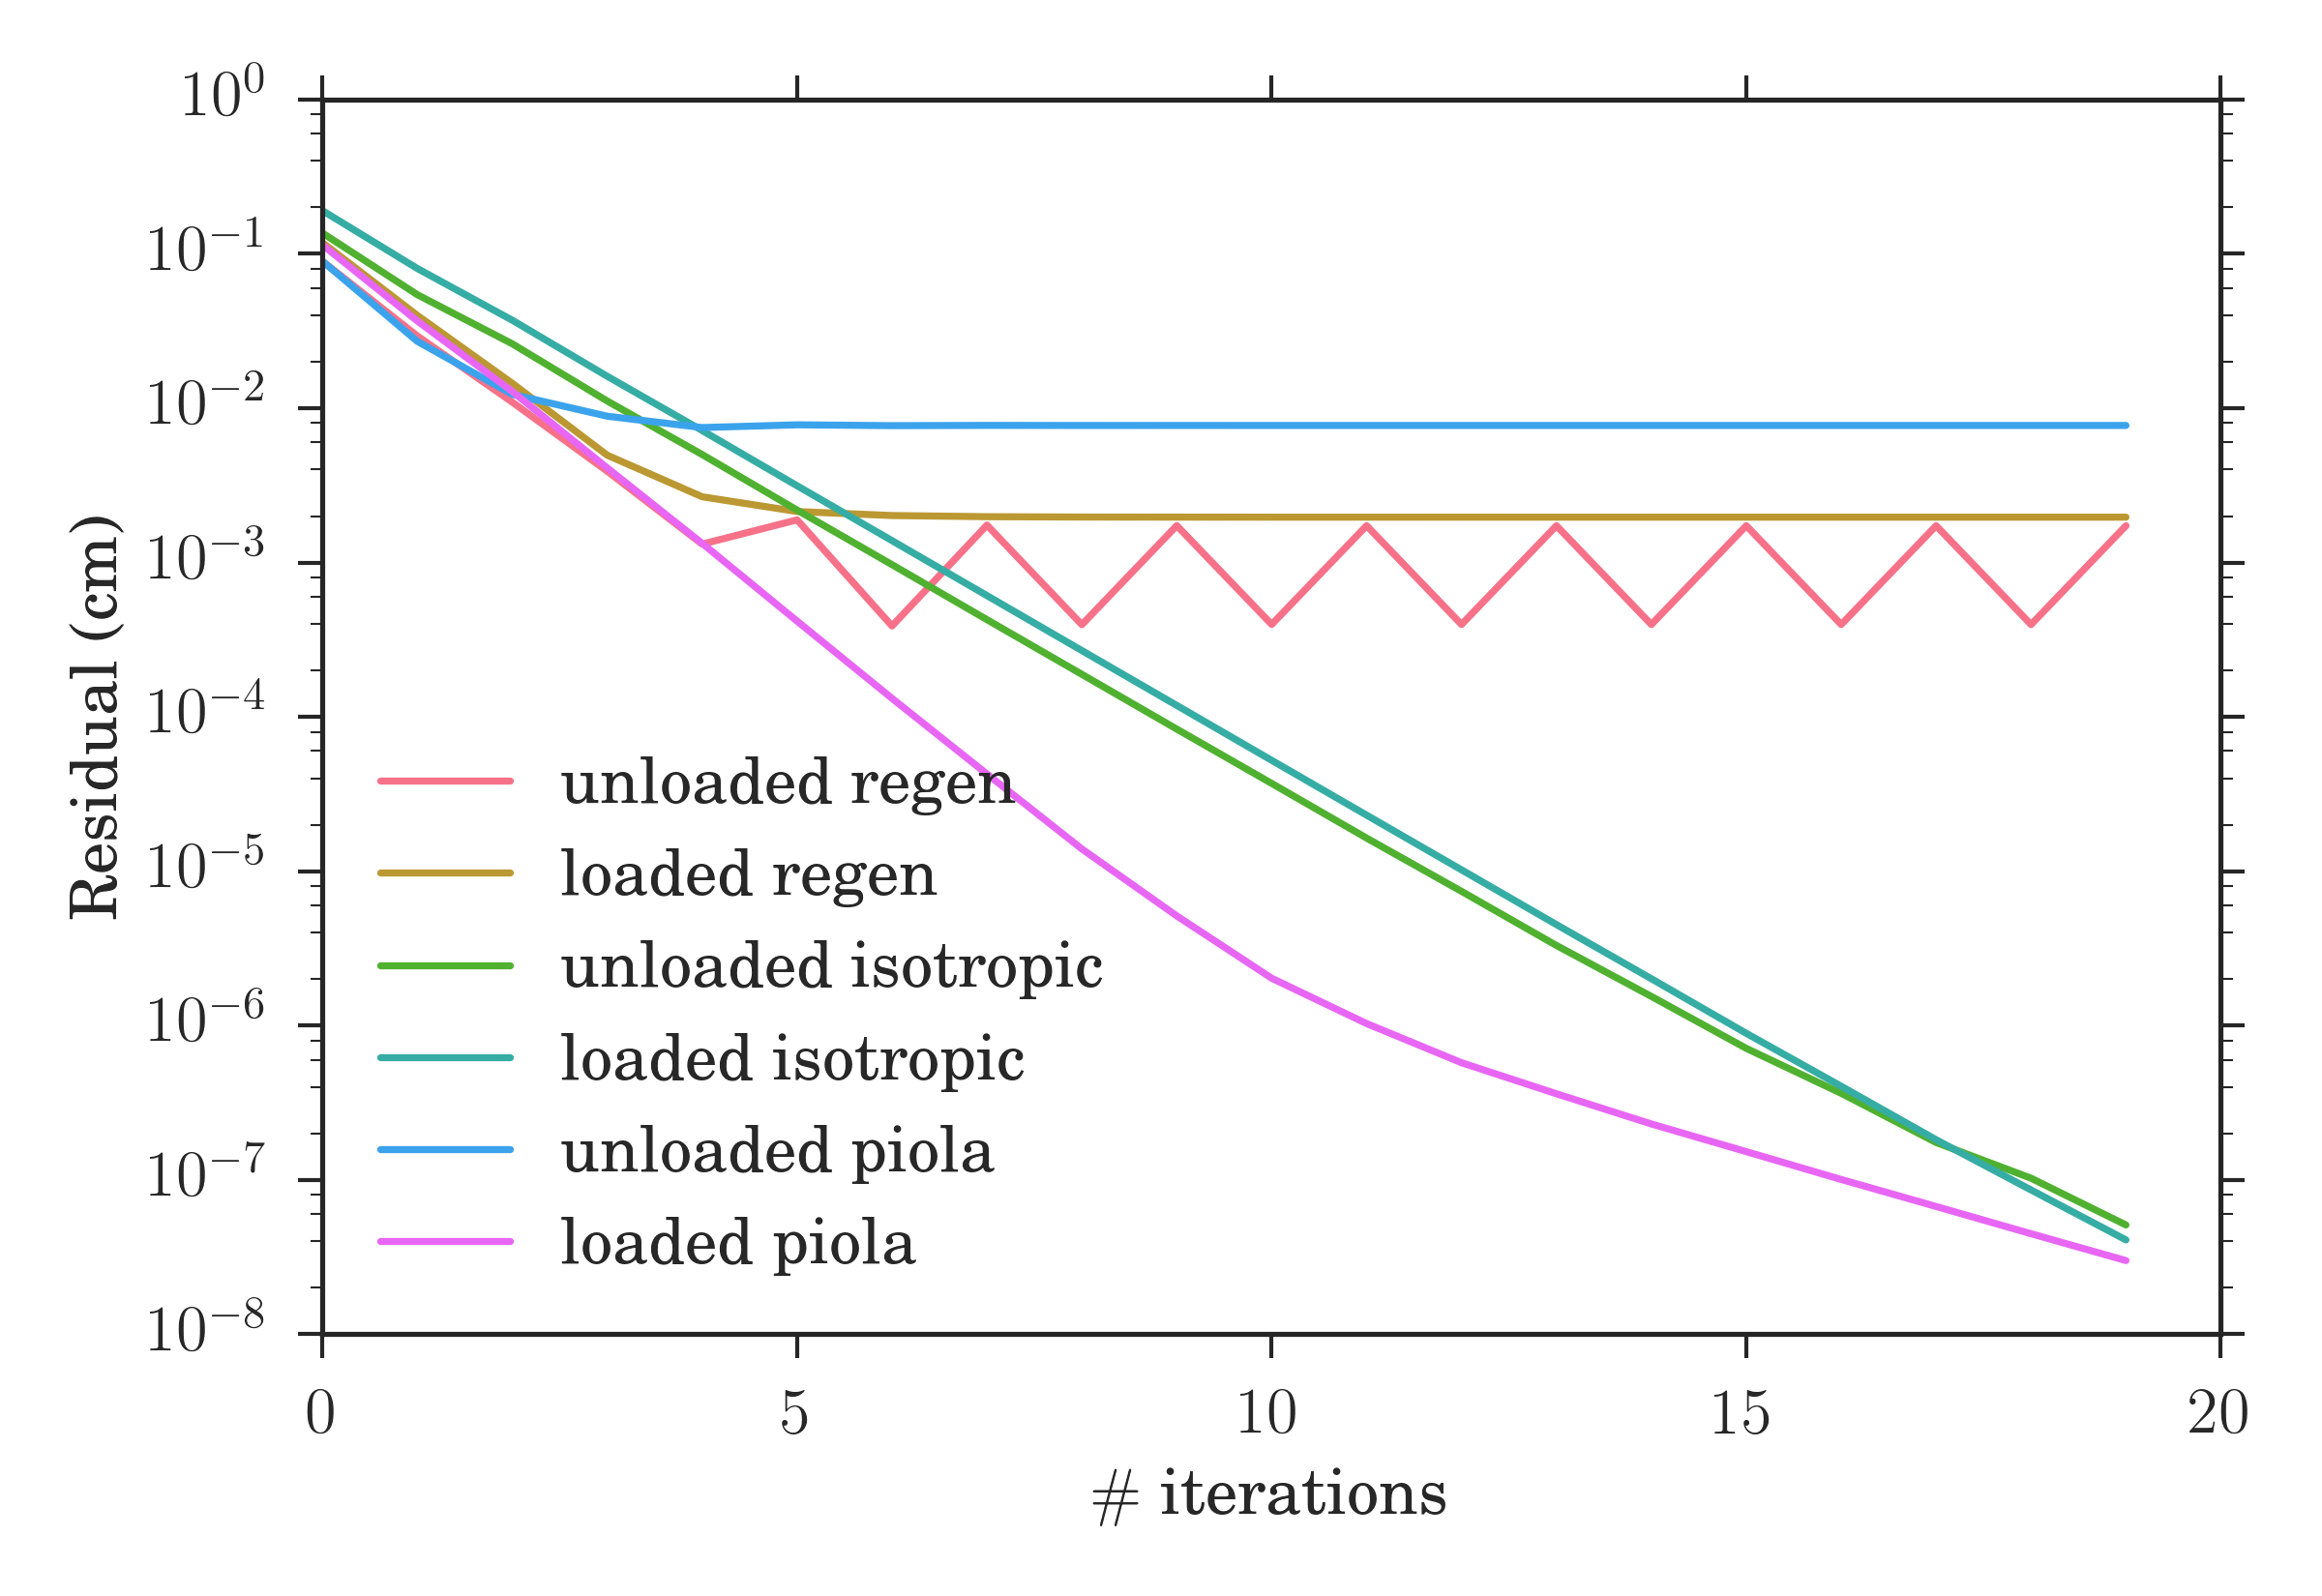
\includegraphics[width=0.7\textwidth]{numerical_experiments/unloading/unloaded_error.png}
\caption{Showing the residual between the known unloaded and estimated
unloaded geometry, and the residual between the loaded geometry and
the image-based geometry. Three different cases are tested; one where
the material is considered isotropic, one with a transversely
isotropic material with fibers mapped to the new reference geometry via
a Piola transformation, and one with a transversely
isotropic material where the fibers are regenerated at
every iteration. }
\label{fig:unloaded_error}
\end{figure}



\section{Parallel Performance}
Write a section here where we test a sample code on multiple cores to
test scalability

Write Short about MPI, and how mesh is distributed on different
cores in FEniCS


\begin{table}
  \centering
    \begin{tabular}{llrrrrr}
\hline
   $\#$ elements & Phase & Serial(s) & 1 core (s)& 2 cores (s) &  4 cores (s)&  8 cores (s)\\
\hline
      \multirow{2}{*}{2095} & passive &   26.605 &   26.605 &   20.147 &  12.75 &   7.8642 \\
                      & active &    40.853 &   40.853 &   29.897 &  18.233 &  11.571 \\
      \multirow{2}{*}{8680} & passive & 223.91  &  223.91  &  226.75  & 117.16 &  71.844  \\
                      & active &   190.16  &  190.16  &  193.19  &  99.312 &  60.043 \\
      \multirow{2}{*}{22623} & passive &   1045.1   & 1045.1   & 1248.5   & 571.26 & 337.21   \\
                         & active &   1123.1   & 1123.1   & 1217.1   & 679.88  & 341.71  \\
\hline
    \end{tabular}
    \caption{\label{}Timings running on different number of cores on a
      single node}
  \end{table}


\begin{table}
  \centering
    \begin{tabular}{llrrrrr}
\hline
   $\#$ elements & Phase & Serial (s)& 1 core (s)& 2 cores (s) &  4 cores (s)&  8 cores (s)\\
\hline
      \multirow{2}{*}{2095} & passive &   26.605 &   25.974 &   20.356 &  11.982 &   8.1715 \\
                      & active &   40.853 &   41.061 &   30.028 &  19.922 &  12.482 \\
      \multirow{2}{*}{8680} & passive & 223.91  &  247.74  &  220.68  & 112.04  &  72.954  \\
                      & active &  190.16  &  184.83  &  192.42  &  96.136 &  62.537 \\
      \multirow{2}{*}{22623} & passive &  1045.1   & 1060.6   & 1228.7   & 611.83  & 343.5    \\
                         & active &  1123.1   & 1062.1   & 1268.6   & 597.21  & 364.52  \\
\hline
    \end{tabular}
    \caption{\label{}Timings running on different number of cores
      on two nodes.}
  \end{table}
